\documentclass[fleqn]{article}

%%%%%%%%%%%%%%%%%%%% PACKAGE SETUP %%%%%%%%%%%%%%%%%%%%
% Packages without explicit setup
\usepackage{amssymb, amsmath}
\usepackage{mathtools}
\usepackage{enumitem}
\usepackage{titlesec}
\usepackage{float}
\usepackage{wrapfig}
\usepackage{multicol}
\usepackage{graphicx}
\usepackage{needspace}
\usepackage{comment}
\usepackage{subcaption}
\usepackage{bm}
\usepackage{hyperref}
\usepackage{multirow}

% Setup the geometry package (for page layout) and spacing.
\usepackage[margin=1.0in]{geometry}

% Setup the hyperref package for clickable links.
\hypersetup{
    colorlinks=true,
    linkcolor=blue,
    filecolor=magenta,      
    urlcolor=blue,
}

\setlength{\parskip}{6pt plus 2pt minus 2pt}
\setlength{\parindent}{0in}

% Load the fancy headers package, using the defaults.
\usepackage{fancyhdr}
\pagestyle{fancy}

% Setup the listings, including using color.
\usepackage{listings}
\usepackage{xcolor}
\lstset{
  showlines   = true,
  numbers     = left,
  frame       = single,
  basicstyle  = \footnotesize\ttfamily,
  basewidth   = 0.5em,
  xleftmargin = 0.33in,
  keywordstyle = \color{blue},
  commentstyle = \color{teal},
  stringstyle  = \color{violet},
}
\lstdefinestyle{continueyellow}{
  firstnumber     = last,
  backgroundcolor = \color{yellow},
  aboveskip       = -\smallskipamount,
}
\lstdefinestyle{continue}{
  firstnumber     = last,
  aboveskip       = -\smallskipamount,
}

% Additional math operators.
\DeclarePairedDelimiter\abs{\lvert}{\rvert}
\DeclarePairedDelimiter\floor{\lfloor}{\rfloor}
\DeclarePairedDelimiter\norm{\lVert}{\rVert}

\DeclareMathOperator{\asin}{asin}
\DeclareMathOperator{\acos}{acos}
\DeclareMathOperator{\atan}{atan}
\DeclareMathOperator{\atantwo}{atan2}	% Using '2' in the operator messes up.

\newcommand{\overbar}[1]{\mkern 1.5mu\overline{\mkern-1.5mu#1\mkern-1.5mu}\mkern 1.5mu}

\usepackage{textcomp, gensymb}
\renewcommand\deg{\degree}


%%%%%%%%%%%%%%%%%%%% START OF DOCUMENT %%%%%%%%%%%%%%%%%%%%
\begin{document}

% Set the header/title.
\fancyhead[L]{ME/CS/EE 133a, Fall 2024-25}
\fancyhead[R]{Git Recitation Notes}
\begin{center}\LARGE Git Recitation Notes \end{center}

\section*{Intoduction - What is Git?}
Git is what's known as a \textit{distributed version control system} or DVCS.
It was invented by Linus Torvalds, the creator of Linux, in 2005 to take the
place of centralized version control systems (CVCS) used by Linux developers.

Version control systems are used to track changes in files and directories over
time. All VCSs have the following elements:

\begin{itemize}
    \item \textbf{Repository:} A database that stores all the changes to files
                               and directories.
    \item \textbf{Working Directory:} A directory on your computer where you can
                                      edit files from the repository.
    \item \textbf{Staging Area:} A cache of changes from the working directory
                                that are ready to be committed.
    \item \textbf{Commit:} A snapshot of the repository at a given time.
    \item \textbf{Commit History:} A log of all the commits that have been
                                   made to the repository.
\end{itemize}

Git, and other DVCS, are distributed in that every user has a complete copy of
the repository on their computer, rather than always relying on a single
central server upstream. This allows for more flexibility and robustness in
collaborative development.

\begin{center}
    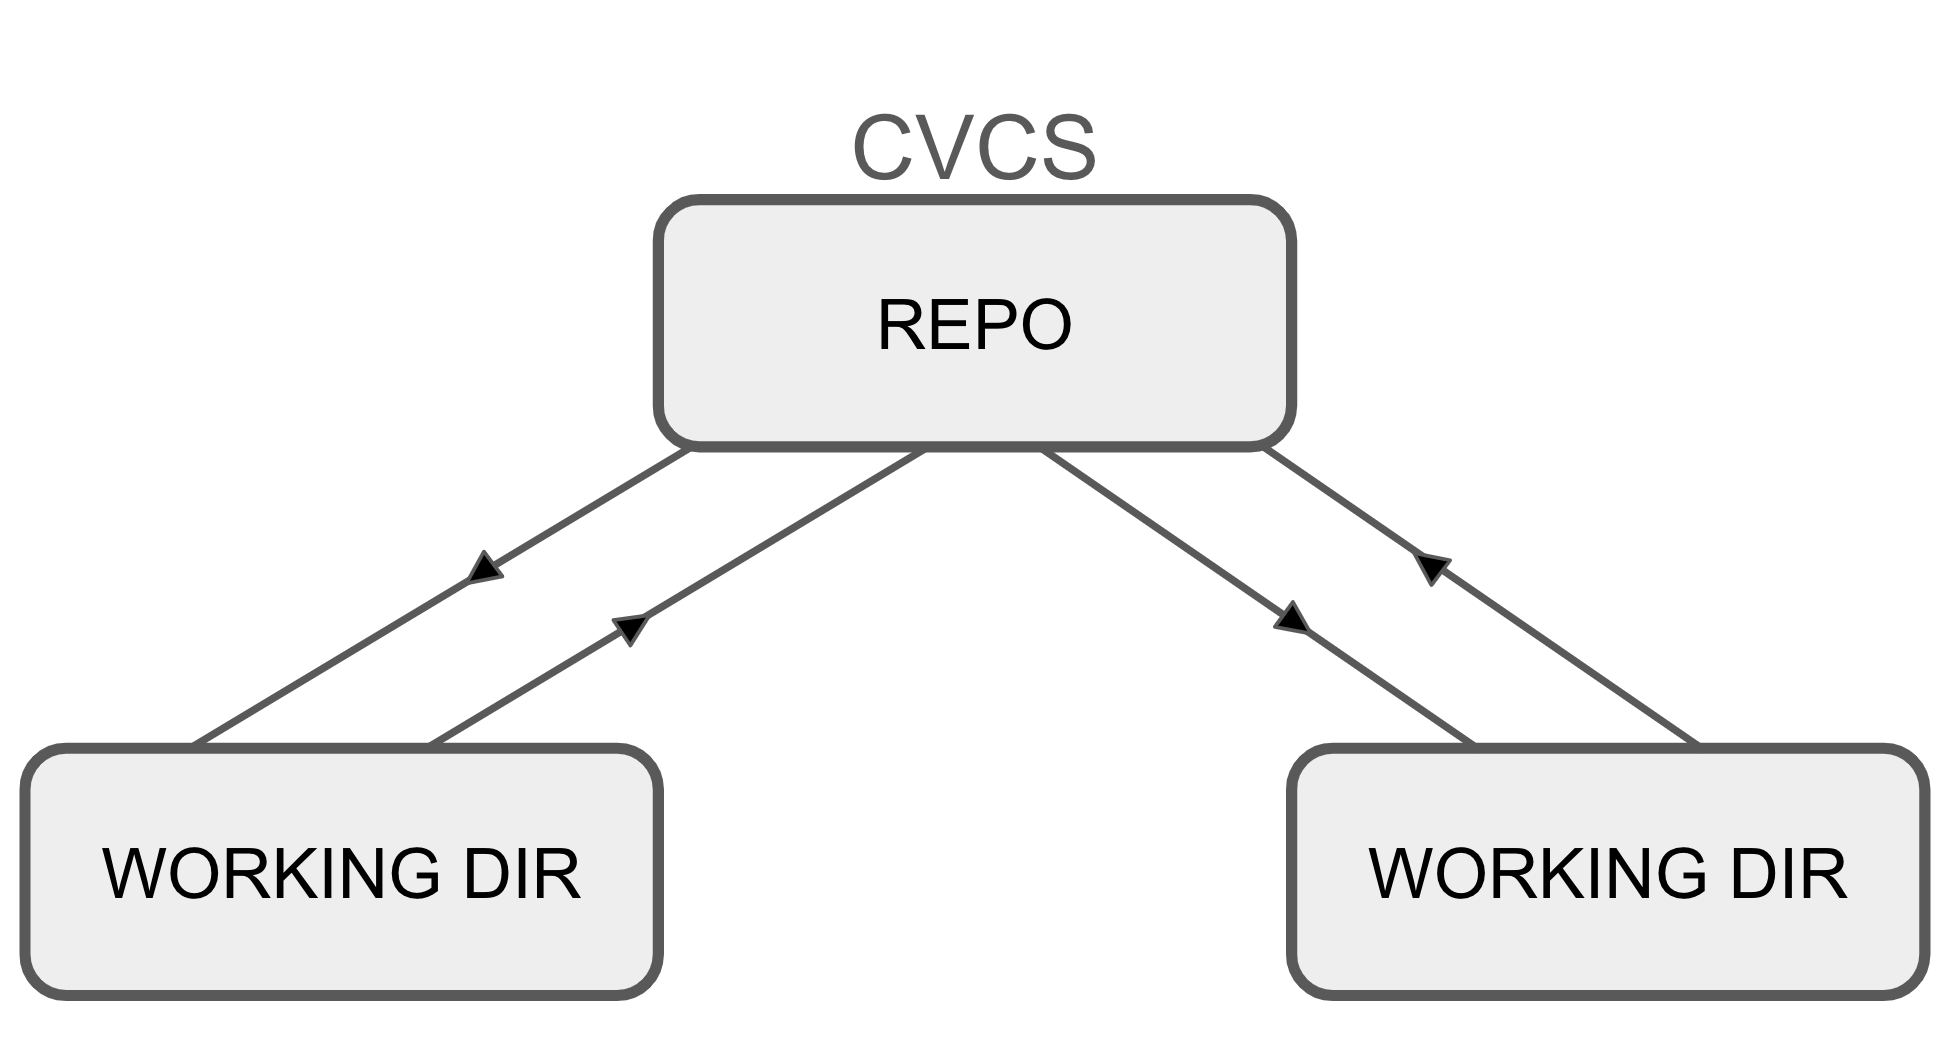
\includegraphics[scale=0.25]{figs/cvcs.png}
    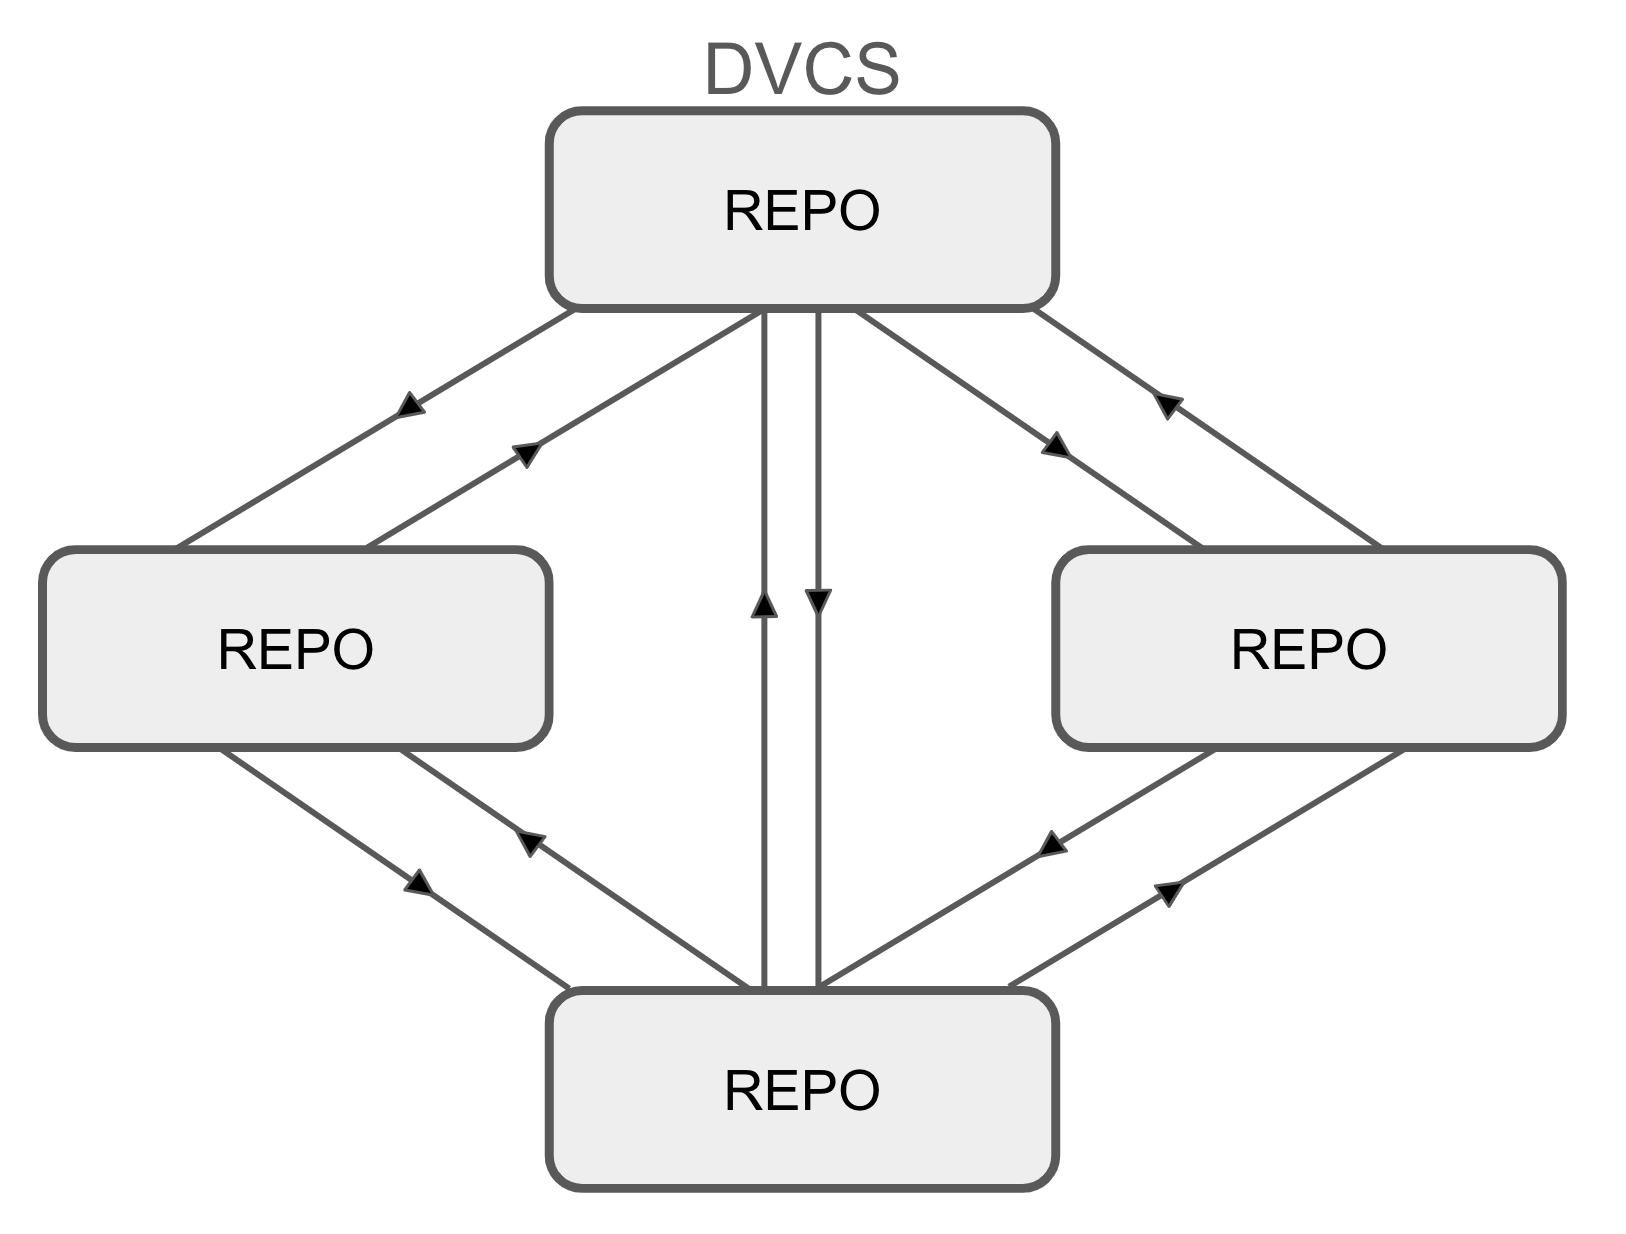
\includegraphics[scale=0.25]{figs/dvcs.png}
\end{center}

The way a DVCS like Git is used is to have a repository hosted on a server - i.e
a repository hosted at \texttt{gitlab.caltech.edu} - which serves as the official
version of the code. Each developer will then clone the repository to their local
machine, work on the code in their working directory, and then upload or
\texttt{push} their changes up to the server. An overview of the git architecture
is show in the following diagram. We will be explaining and understanding each
component of this diagram as we go:

\begin{center}
    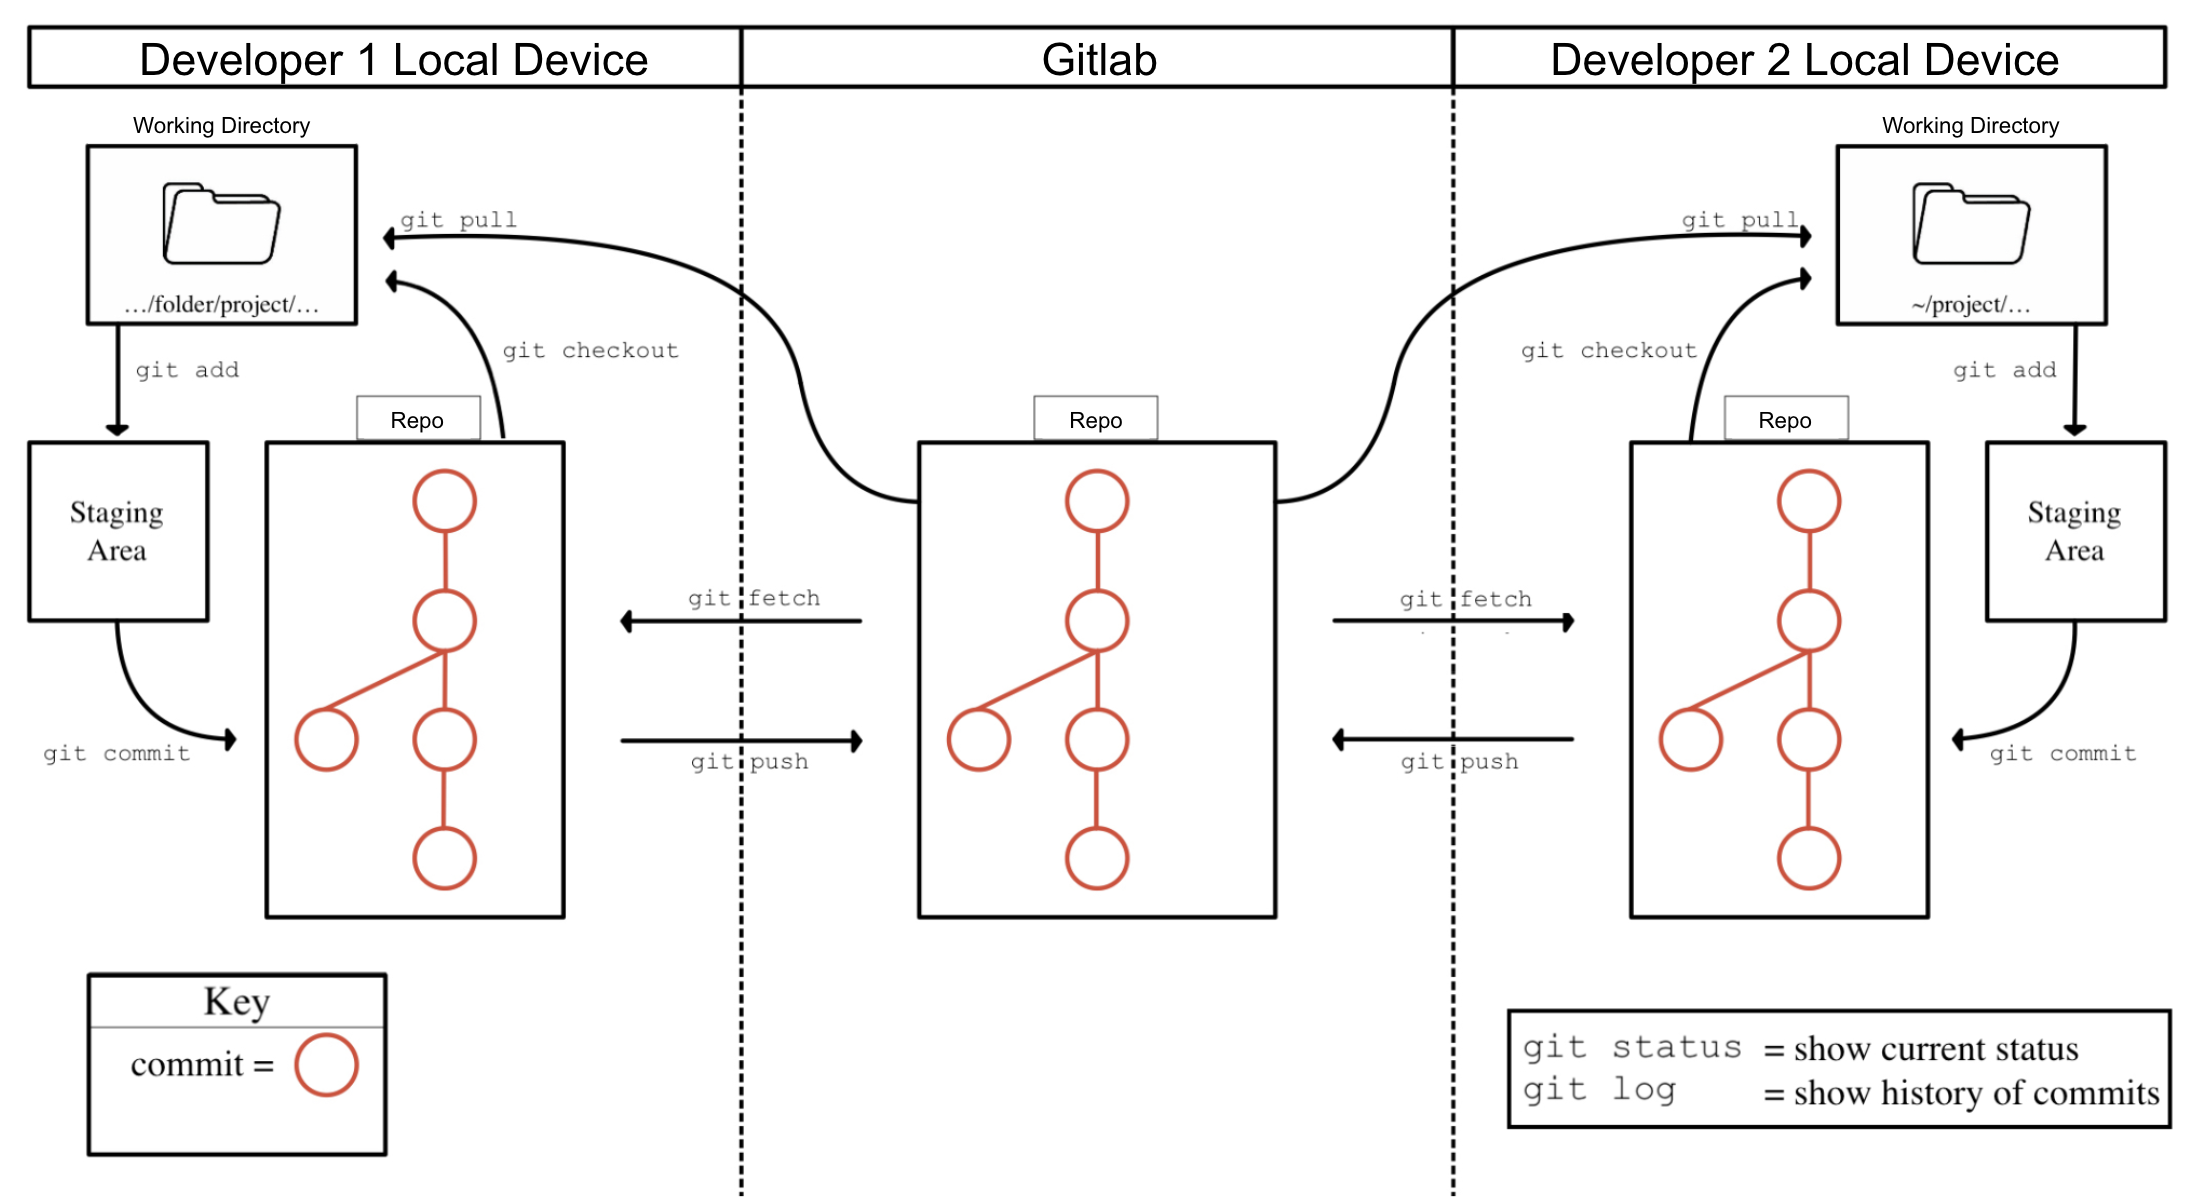
\includegraphics[scale=0.4]{figs/overview.png}
\end{center}

\section*{Setting Up - Git Config}

Before you start using Git, there are a few things you need to do. First, check
that git is installed on your computer by running:

\begin{lstlisting}
git --version
\end{lstlisting}

If you don't have git installed, you can download it from the Git website. Once
you have git installed, you need to configure it with your name and email. This
is important because every commit you make will have this information attached
to it, and it will identify to the server who you are when you want to push your
changes. To set your name and email:

\begin{lstlisting}
git config --global user.name "Your Name"
git config --global user.email "
\end{lstlisting}

These commands will add your information to your global git configuration file,
which is located at \texttt{\textasciitilde/.gitconfig} on Unix systems and
\texttt{C:\textbackslash Users\textbackslash username\textbackslash .gitconfig}
on Windows systems.

You will also need to set up an SSH key to authenticate with the remote
repository. Follow the instruction given
\href{https://docs.gitlab.com/ee/user/ssh.html}{here} to set up an SSH key for
your GitLab account.

You're now ready to clone a repository from Gitlab and begin working!

\pagebreak

\section*{Committing}
The most basic operation in Git is committing. This is the process of taking a
snapshot of the repository at a given time, including all of the changes that 
have been moved from the working directory to the staging area. Every commit
has the following elements:

\begin{itemize}
    \item \textbf{Author:} The person who made the commit.
    \item \textbf{Date:} The date and time the commit was made.
    \item \textbf{Message:} A short description of the changes made in the
                            commit.
    \item \textbf{Hash:} A unique identifier computed for the commit.
\end{itemize}

To add your changes to the staging area:
\begin{lstlisting}
git add <filepath>  # Add a single file
git add <directory> # Add all files under a directory
git add .           # Add all files under the working directory
\end{lstlisting}

To commit your changes to the repository:
\begin{lstlisting}
git commit -m <Your commit message here>
\end{lstlisting}

It may be useful to see the history of commits in the repository, who made them,
and what the message on each commit is. To do this:

\begin{lstlisting}
git log                        # See a detailed log of all commits
git log --oneline              # See a one-line summary of each commit
git log -n <number of commits> # See the last n commits
\end{lstlisting}

It may also be useful to see the differences between two commits, or between
the working directory and a commit. To do so:

\begin{lstlisting}
git diff                             # Compare the working directory to the staging area
git diff <commit hash>               # Compare a commit to the working directory
git diff <commit hash> <commit hash> # Compare two commits
\end{lstlisting}

To see your current status, including which files are staged, unstaged changes,
and much more that will make sense as you get more familiar with Git:

\begin{lstlisting}
git status
\end{lstlisting}

Finally, you may want to reset certain files or the entire repository to a
previous commit (notice that you CAN LOSE WORK this way if you aren't careful):

\begin{lstlisting}
git reset HEAD             # Reset the staging area to the last commit
git reset HEAD <filepath>  # Reset a single file in the staging area
git reset --hard HEAD      # Reset the entire repository to the last commit
git reset --hard HEAD~<n>  # Reset the entire repository to n commits ago
git reset --hard <commit>  # Reset the entire repository to a specific commit
\end{lstlisting}

\pagebreak

\section*{Branching}

Using a DVCS like Git allows users to create branches, which are separate
commit histories split off from a commmon origin that can be worked on
independently. 

\begin{center}
    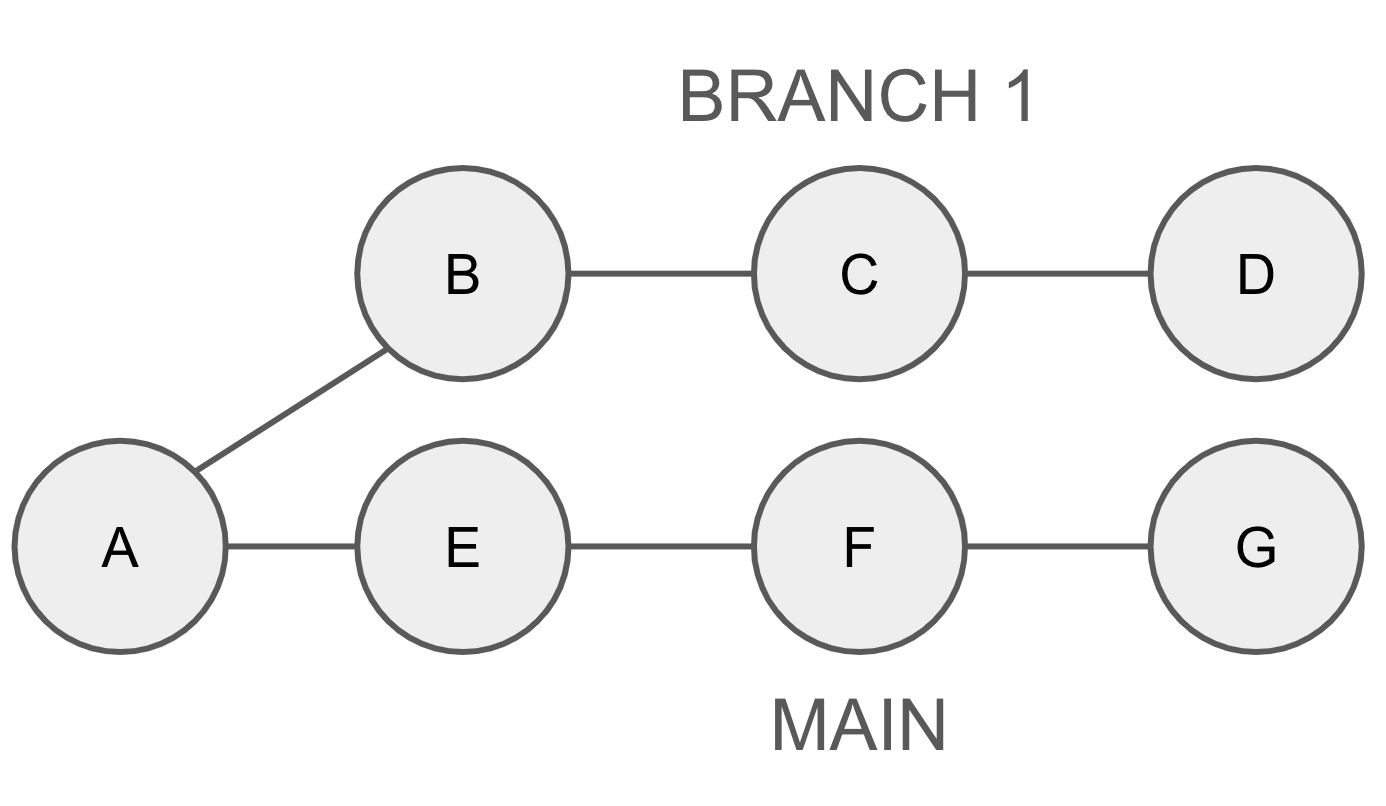
\includegraphics[scale=0.3]{figs/branch.png}
\end{center}

The HEAD pointer in Git is a reference to the current branch you are working on.
This means that your working directory will reflect the state of the branch
that HEAD is pointing to. Placing the head pointer on a branch is called
checking out a branch.

To see the current branch and the branches that exist in the repository:

\begin{lstlisting}
git branch
\end{lstlisting}

To create a new branch:

\begin{lstlisting}
git branch <branchname>        # Create a new branch but don't check it out
git checkout -b  <branchname>  # Create a new branch and check it out
\end{lstlisting}

To switch to a different branch:

\begin{lstlisting}
git checkout <branchname> # Switch to an existing local branch
git switch   <branchname> # Switch to an existing remote branch
\end{lstlisting}

Very often, you will want to merge the changes from one branch into another. 
For example, say I branched off from the main branch and added a new feature 
to my code. I now need to merge my changes back into main. To do this:

\begin{lstlisting}
git checkout main
git merge <branchname>
\end{lstlisting}

\begin{center}
    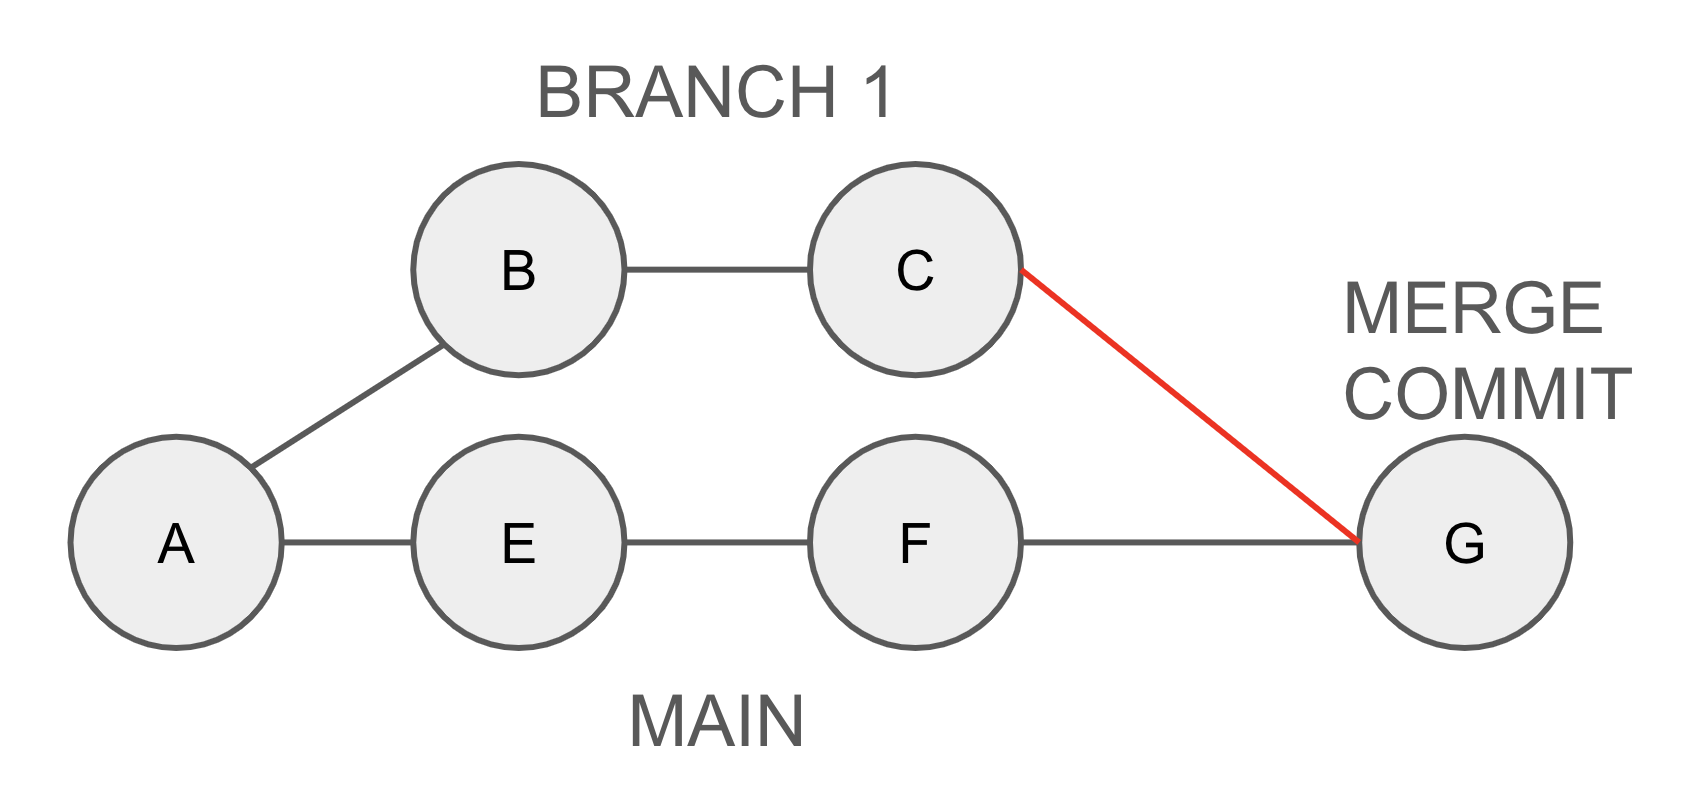
\includegraphics[scale=0.3]{figs/merge.png}
\end{center}

What if someone else added some changes to the main branch while I was working
on my feature? This is where merge conflicts can arise. Git will try to merge
the changes automatically, but if it can't, it will ask you to resolve the
conflict manually.

\pagebreak

\section*{Stashing}

Sometimes while working, you may run into the following situations:
\begin{itemize}
    \item You want to run the code from your latest commit, but you have
          uncommitted changes in your working directory.
    \item You want to switch to a different branch, but you have uncommitted
          changes in your working directory.
    \item You accidentally edited on the wrong branch, and you need to move your
          changes to a different branch.
    \item You want to see what your code looked like before you edited it, and
          the output of \texttt{git diff} is annoying to read.
\end{itemize}

In these use cases, and in more (any time you want to save your changes without
committing them), you can use the \texttt{git stash} command. The Git stash is 
a LIFO stack that allows you to save your changes and restore them later
without committing them or making a seperate branch.

For example:

\begin{lstlisting}
git checkout main                    # Switch to the main branch
vim hello_world.py                   # Make some changes to a file

(OOPS I want to run the old version)

git stash push                       # Save your changes to the stash
python hello_world.py                # Run the old version of the code
git stash pop                        # Restore your changes from the stash
\end{lstlisting}

\begin{lstlisting}
git checkout main                   # Switch to the main branch

(work on main with unsaved changes) # OOPS I meant to work on my feature branch

git stash                           # Save your changes to the stash
git checkout <branchname>           # Switch to your feature branch
git stash pop                       # Restore your changes from the stash
\end{lstlisting}

In this example, as is always the case with git, there could be merge conflicts
to resolve when you apply the changes from the most recent stash entry to your
working directory.

Keep in mind that the stash can have many entries in it. I recommend adding a
message to your stash entries to keep track of what you are stashing. You can 
see a list of all our your stash entries and their associated messages using
\texttt{git stash list}.

\begin{lstlisting}
git stash push -m <commit message>  # Stash your changes with a message
git stash list                      # List all your stash entries
\end{lstlisting}

You can also appply changes from a specific stash entry not at the top of the
stash using \texttt{git stash apply}. You refer to each entry as
\texttt{stash@n}, where \texttt{n} is the 0-indexed index of the stash entry.
For example, to apply the second stash entry:

\begin{lstlisting}
git stash apply stash@{1}  # Apply the second stash entry
\end{lstlisting}

To delete an old entry from the stash that you don't need anymore:

\begin{lstlisting}
git stash drop stash@{1}  # Delete the second stash entry
\end{lstlisting}

\pagebreak

\section*{Rebasing}

Rebasing is another way to integrate changes from one branch into another
besides merging. It works by moving the commits from one branch to another, and
then replaying the commits on top of the branch you are rebasing onto. For
example, say you have a feature branch that you aren't ready to merge into main
yet, but you want to keep it up to date with the main branch. You can rebase the
feature branch onto the main branch to incorporate the changes from main.

\begin{center}
    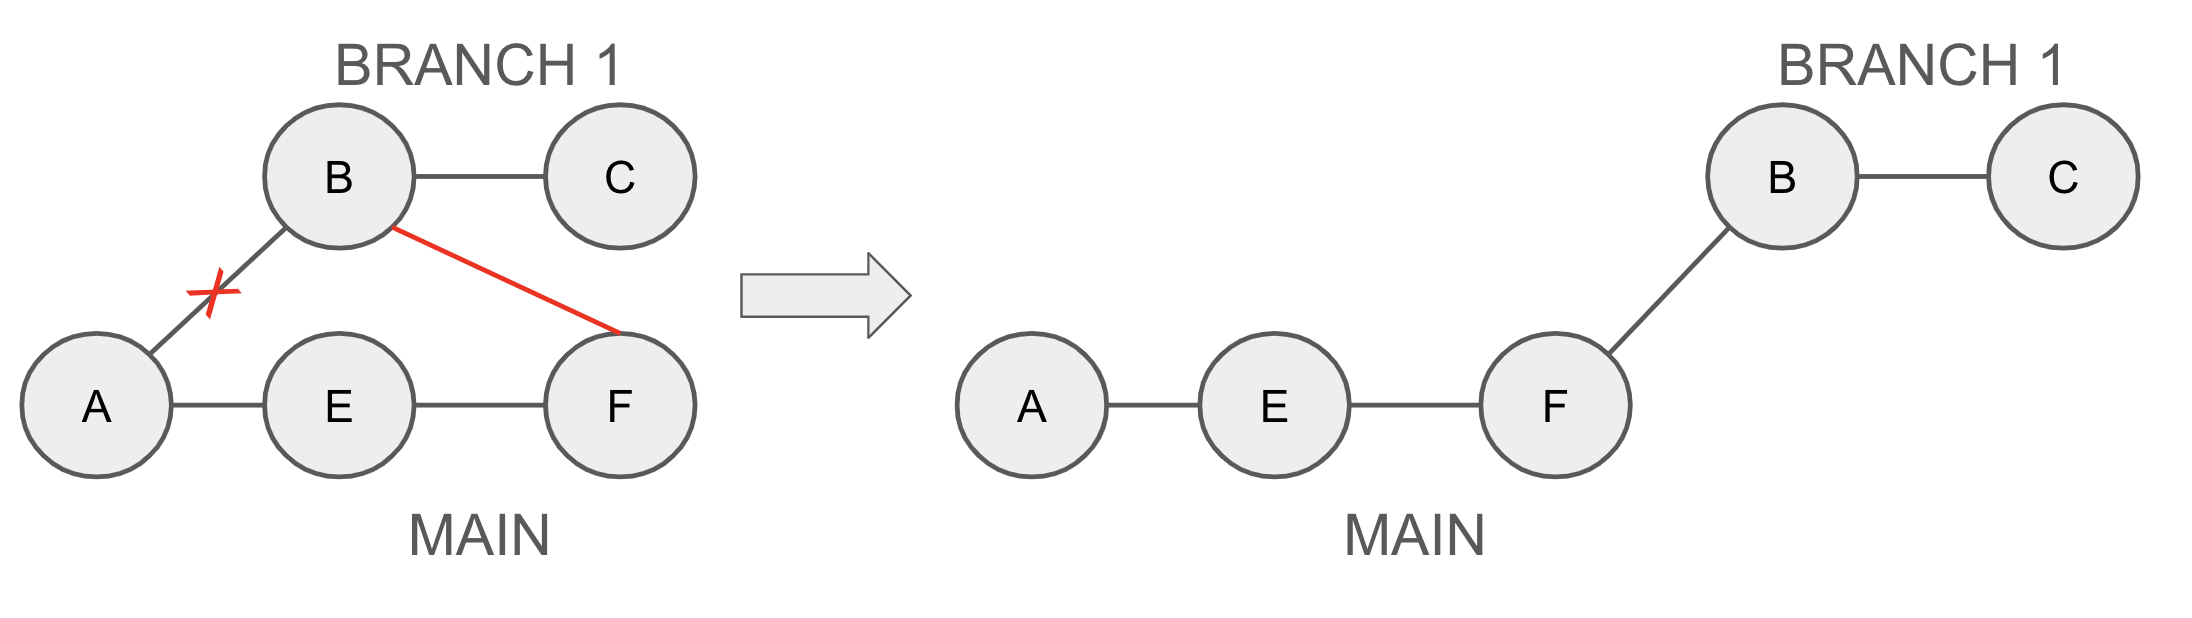
\includegraphics[scale=0.4]{figs/rebase.png}
\end{center}

Rebasing can be risky because it rewrites the commit history of the branch you
are rebasing. This can cause problems if you are working on a branch that is
shared with other people. I recommend always backing up your branch before 
attemping a rebase. To backup your branch:

\begin{lstlisting}
git branch my_backup_branch
\end{lstlisting}

To rebase your branch onto another branch:

\begin{lstlisting}
git checkout <branchname>
git rebase <branchname>
\end{lstlisting}

A powerful type of rebase is an interactive rebase. This allows you to edit,
squash, or delete commits at will as you rebase. To do this:

\begin{lstlisting}
git rebase -i <branchname>             # Rebase onto another branch
git rebase -i HEAD~<number of commits> # Rebase onto the last n commits
git rebase -i <commit hash>            # Rebase onto a specific commit
\end{lstlisting}

These commands will open a text editor with a list of commits that you can
edit. You can change the order of commits, squash commits together, or delete
commits entirely. The text editor will include instructions on how to do this.

\pagebreak

\section*{Remote Repositories}

So far, we have only been working with a local repository on our computer.
However, Git is designed to work with remote repositories as well. A remote
repository is a copy of the repository that is stored on a server, and can be
accessed by multiple users. The most common way to interact with a remote
repository is through a web service. For us, this will be GitLab.

To copy a remote repository to your local machine:

\begin{lstlisting}
git clone <repository URL>
\end{lstlisting}

This will automatically add the remote repository as a remote called
\texttt{origin}.

Note that you may have to set up authentication to access the remote repository.
This is done using an SSH key, and you should find instructions on how to do
this in the documentation of the service you are using.

Say instead that you have a local repository and you want to add a remote
repository to it. To do this:

\begin{lstlisting}
git remote add <remote name> <repository URL>
\end{lstlisting}

By convention, the main remote should be named \texttt{origin}. By the power of
DVCS, you can have multiple remotes for a single repository.

In a simple workflow, you may not need to use multiple branches. In this case,
you may simply edit files in the working directory on the \texttt{main} branch,
add and commit changes, and push them to the remote repository.

\begin{lstlisting}
git pull                       # Pull changes on main from the remote repository

(Work on main branch)

git add .                      # Add changes to the staging area
git commit -m <commit message> # Commit changes to the repository
git push                       # Push changes on main to the remote repository
\end{lstlisting}

If you want to sync your local repository with the remote repository without
making changes to your working directory you can use \texttt{git fetch}. This
means you can check to see if there are any changes on the remote that you need
to rebase onto, or if you need to pull changes from the remote.

Remember that with a DVCS, you have a complete copy of the repository on your
local machine. This means that your local repository can have multiple branches
that are not present in the remote repository. To synchronize your local
branches with the remote repository, you set an upstream branch.
This is a mapping between a local branch and a remote branch. Once an
upstream is set, you use \texttt{git push} to push changes to the remote
branch, and \texttt{git pull} to pull changes from the remote branch.

Take the following example of a slightly more complex workflow:

\begin{lstlisting}
git clone <repository URL>    # Clone repo from remote
git checkout -b feature       # Create a new feature branch locally

(Work on feature branch)

git push -u origin feature    # Push changes to remote and set upstream

(Work on feature branch more)

git push                      # Push changes to remote (upstream already set)
git push -f                   # Push changes to remote if you have divergent histories
\end{lstlisting}

It's best practice to push your new commits to the remote frequently as a 
backup mechanism. This way, if your computer crashes, you won't lose your work.

When you are ready to merge your branch into the main branch on the remote, you
do so by creating a \emph{pull request} or PR. This is a request to the owner
of the main branch to merge your changes into the main branch, which will be
reviewed through the PR interface on the remote repository. The PR interface
will allow you to see the changes that will be made and conduct code reviews and
discussions with other developers.

\pagebreak

\section*{Simple Workflow - Single Developer or Group Programming}

If all developers are working together on the same code at the same time, we can
use a simple workflow that involves only the \texttt{main} branch. Without
working on multiple feature in parallel, we don't have to worry about merge
conflicts, rebasing, or pull requests. In this workflow:

\begin{enumerate}
    \item Clone the repository to your local machine.
    \item Work on the code in the working directory.
    \item Add changes to the staging area and commit them.
    \item Push changes to the remote repository.
    \item Anytime changes were pushed to the remote from another device, be sure
          to \texttt{git pull} them down to your local repository before making
          more changes.
\end{enumerate}

\section*{Typical Workflow}

The industry-standard workflow (called feature branching) for using Git in a
collaborative environment is as follows:

\begin{enumerate}

    \item Create a remote repository on a service like Github, whose main
          \texttt{main} branch serves as the official version of the code.
    \item Each team member clones the repository to their local machine.
    \item Each team member works on new features of the code in parallel, in
          their own branches.
    \item Each team member pushes their changes to a new branch on the remote
          set as the upstream of their branch.
    \item Each team member creates a pull request to merge their branch into
          the main branch.
    \item The branch is reviewed by other team members, who can leave comments
          and request changes.
    \item Once a team member's pull request is approved, they rebase their
          branch onto the main branch to incorporate any changes that have been
          made since they branched off, and  \emph{squash} their changes into a
          single commit (using an interactive rebase).
    \item The team member then merges their branch into the main branch.
\end{enumerate}

\section*{Conclusion}

Git is a powerful tool that can be used to manage changes to code in a
collaborative environment. It is important to understand the basic commands
and concepts of Git in order to use it effectively. The best way to learn Git
is to use it, so I encourage you to practice using best Git practices in your
upcoming final projects. There are many more advanced features of Git that I
have not covered in this recitation, so I encourage you to explore the Git
documentation to learn more. If you get stuck or have any trouble with Git
during the projects, don't hesitate to ask me for help!

\end{document}
